
\section{Results}
\label{sec:experiments}


\begin{figure}[t]
  \centering
  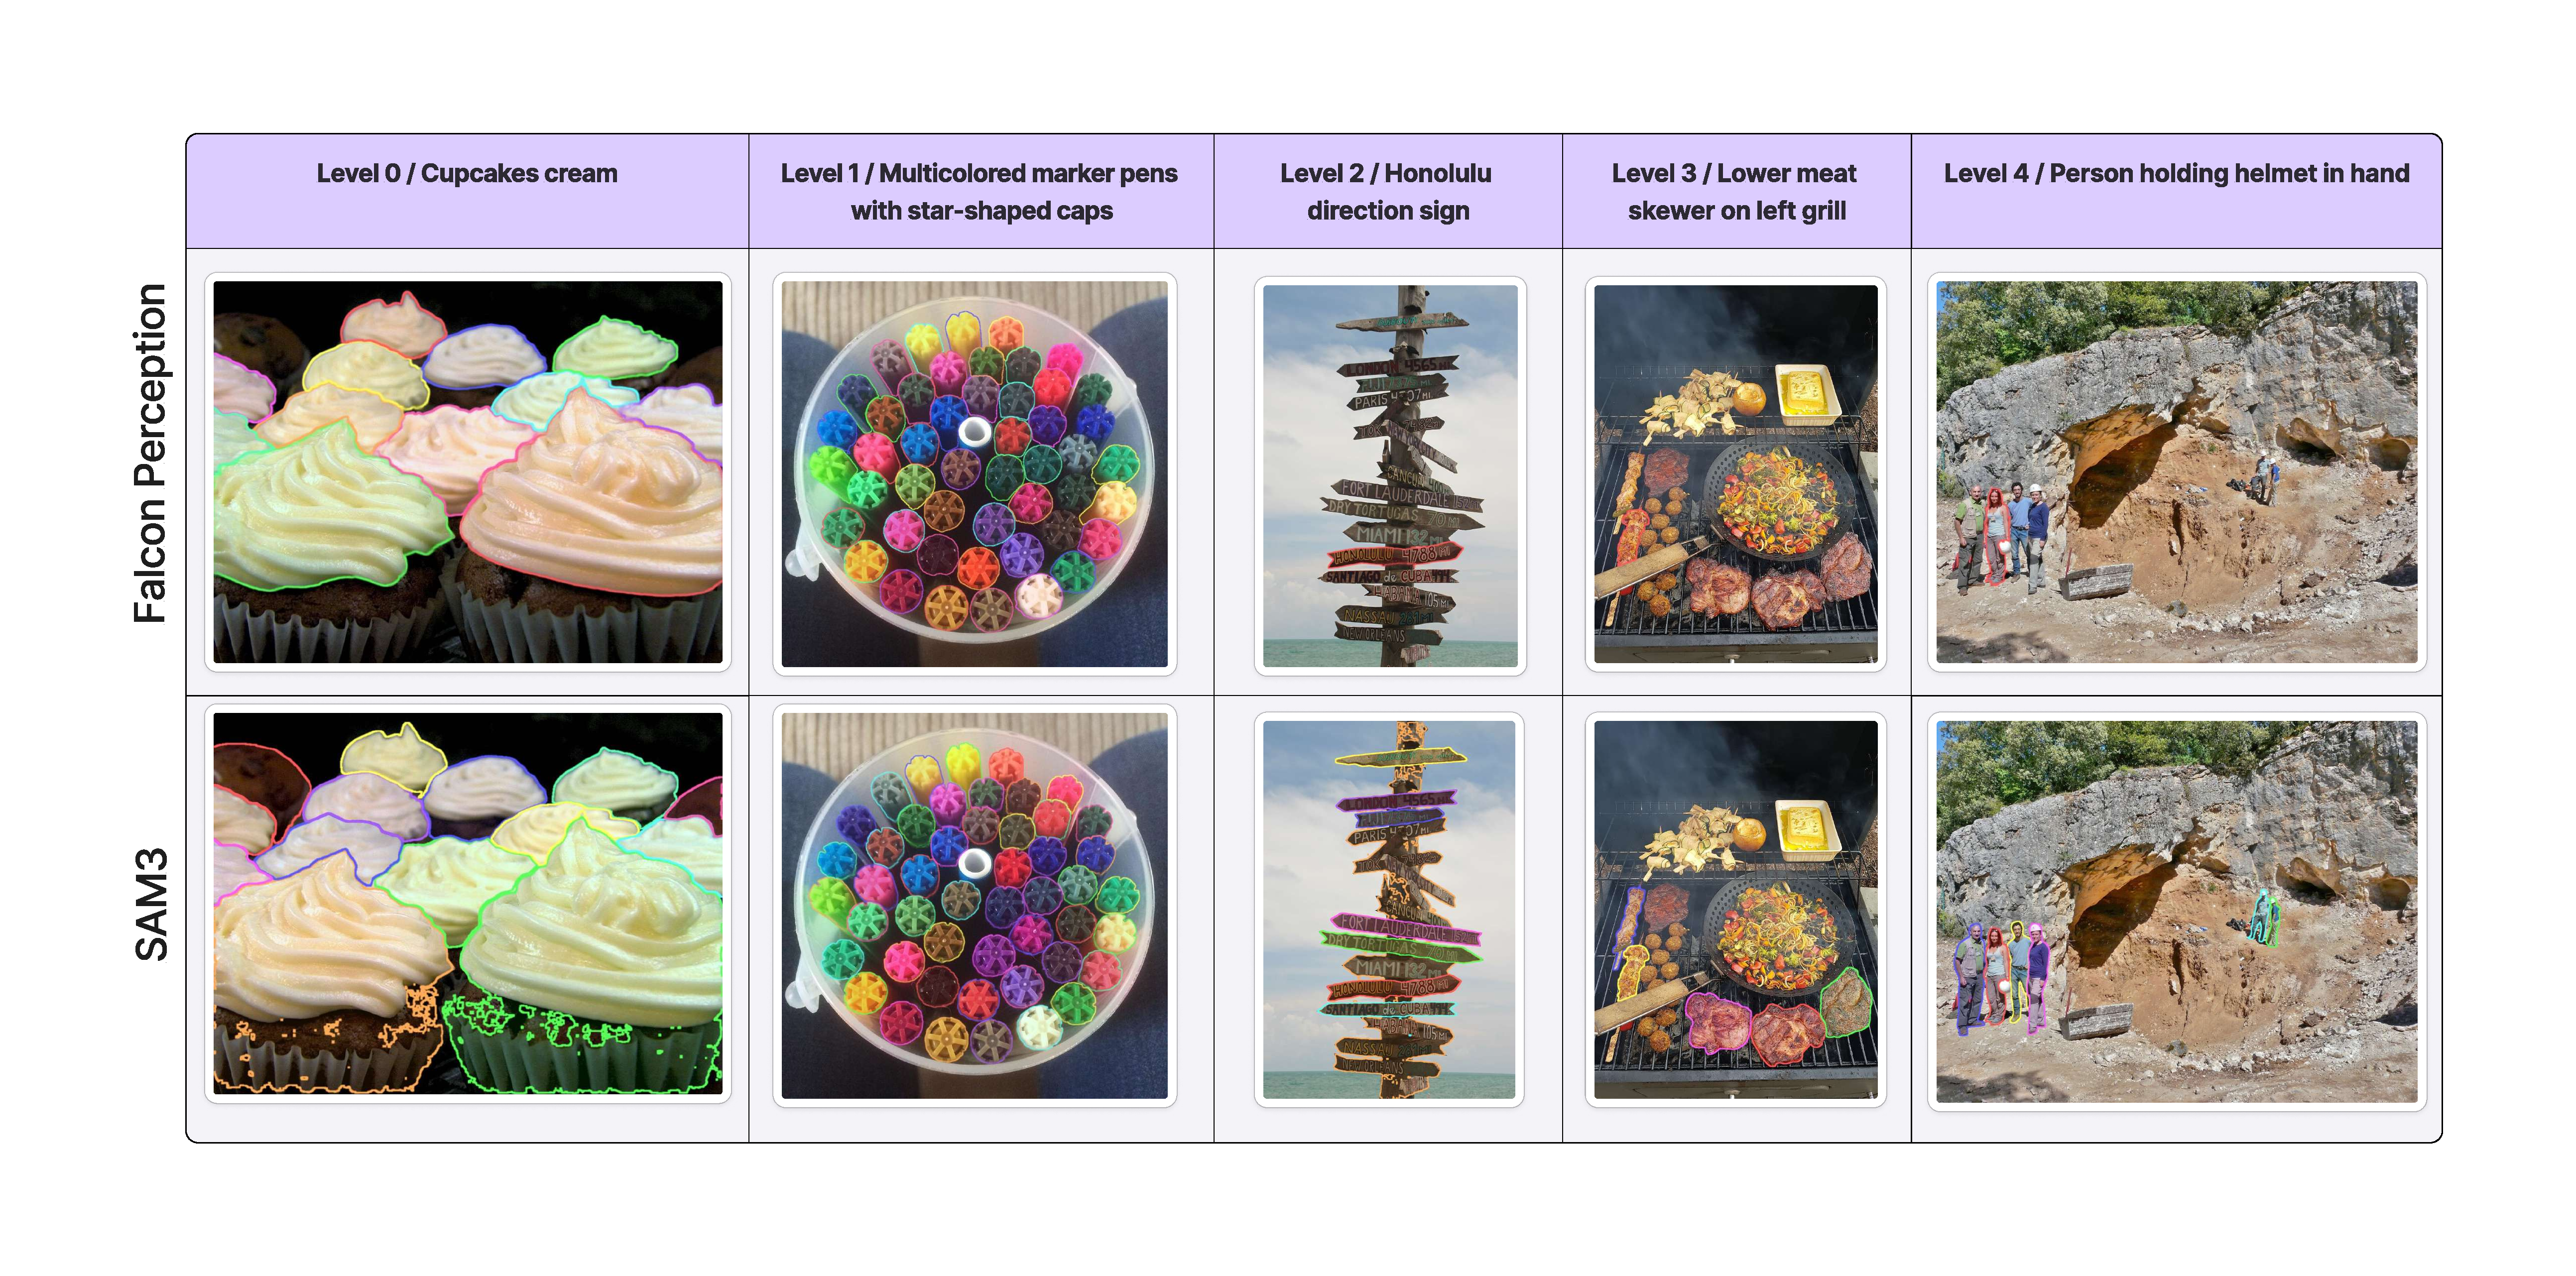
\includegraphics[width=1.0\textwidth, trim=4.5cm 4.5cm 4.5cm 4.5cm, clip]{figures/results_main.pdf}

\caption{\textbf{Qualitative comparison across PBench complexity levels.} Each column shows a different image and a prompt written to target one dominant capability (Levels~0--4; Table~\ref{tab:complexity_levels})). The top row shows Falcon Perception predictions and the bottom row shows SAM~3. Falcon Perception produces cleaner, more instance-specific masks as prompts become more compositional (OCR, spatial, relational), while SAM~3 more often fragments the target or returns extra/incorrect masks on higher-level prompts.}

\label{fig:main_result}
\end{figure}





\begin{table}[t]
    \centering
    \caption{\textbf{SA-Co Benchmark Results.} Comparison of Falcon Perception against state-of-the-art open-vocabulary segmentation models. We report Macro F$_1$, Positive Micro F$_1$ (pmF$_1$), and Image-Level MCC across all splits.\vspace{-0.2cm}}
    \label{tab:saco_results_booktabs}
    \resizebox{\textwidth}{!}{
    \begin{tabular}{l | ccc | ccc | ccc | ccc | ccc | ccc | ccc | ccc}
    \toprule
    \multirow{2}{*}{\textbf{Model}} & \multicolumn{3}{c}{\textbf{Average}} & \multicolumn{3}{c}{\textbf{Metaclip}} & \multicolumn{3}{c}{\textbf{SA-1B}} & \multicolumn{3}{c}{\textbf{Crowded}} & \multicolumn{3}{c}{\textbf{Food\&Drink}} & \multicolumn{3}{c}{\textbf{Sports Equip.}} & \multicolumn{3}{c}{\textbf{Attributes}} & \multicolumn{3}{c}{\textbf{Wiki-Common}} \\
    \cmidrule(lr){2-4} \cmidrule(lr){5-7} \cmidrule(lr){8-10} \cmidrule(lr){11-13} \cmidrule(lr){14-16} \cmidrule(lr){17-19} \cmidrule(lr){20-22} \cmidrule(lr){23-25}
    & F$_1$ & pmF$_1$ & MCC & F$_1$ & pmF$_1$ & MCC & F$_1$ & pmF$_1$ & MCC & F$_1$ & pmF$_1$ & MCC & F$_1$ & pmF$_1$ & MCC & F$_1$ & pmF$_1$ & MCC & F$_1$ & pmF$_1$ & MCC & F$_1$ & pmF$_1$ & MCC \\
    
    \midrule
    \multicolumn{25}{l}{\cellcolor{gray!10}\textbf{Baselines}} \\
    \quad gDino-T~\cite{Liu2023GroundingDM} & - & 16.2 & 0.15 & - & 13.9 & 0.21 & - & 15.4 & 0.20 & - & 3.4 & 0.08 & - & 9.8 & 0.10 & - & 11.2 & 0.10 & - & 47.3 & 0.29 & - & 12.1 & 0.06 \\
    \quad OWLv2*~\cite{minderer2024scalingopenvocabularyobjectdetection} & - & 42.0 & 0.57 & - & 34.3 & 0.52 & - & 26.8 & 0.50 & - & 30.7 & 0.51 & - & 49.4 & 0.65 & - & 56.2 & 0.64 & - & 56.2 & 0.63 & - & 40.3 & 0.54 \\
    \quad OWLv2~\cite{minderer2024scalingopenvocabularyobjectdetection} & - & 36.8 & 0.46 & - & 31.3 & 0.39 & - & 21.7 & 0.45 & - & 24.8 & 0.36 & - & 47.9 & 0.51 & - & 47.0 & 0.52 & - & 48.2 & 0.54 & - & 36.6 & 0.49 \\
    \quad LLMDet-L~\cite{fu2025llmdet} & - & 27.3 & 0.21 & - & 19.4 & 0.23 & - & 22.8 & 0.23 & - & 13.7 & 0.18 & - & 29.1 & 0.19 & - & 25.3 & 0.17 & - & 57.1 & 0.39 & - & 23.3 & 0.16 \\
    \quad APE-D~\cite{shen2024aligning} & - & 36.9 & 0.40 & - & 30.1 & 0.42 & - & 10.0 & 0.22 & - & 20.3 & 0.35 & - & 45.0 & 0.51 & - & 56.5 & 0.56 & - & 57.3 & 0.47 & - & 39.5 & 0.41 \\
    \quad DINO-X~\cite{ren2024dino} & - & 55.2 & 0.38 & - & 49.2 & 0.35 & - & 40.9 & 0.48 & - & 37.5 & 0.34 & - & 61.7 & 0.49 & - & 69.4 & 0.41 & - & \textbf{74.0} & 0.42 & - & 53.5 & 0.35 \\
    
    \midrule
    \multicolumn{25}{l}{\cellcolor{gray!10}\textbf{Vision-Language Models}} \\
    \quad Gemini 2.5~\cite{comanici2025gemini} & - & 46.1 & 0.29 & - & 33.8 & 0.29 & - & 32.1 & 0.41 & - & 30.3 & 0.27 & - & 59.5 & 0.33 & - & 53.5 & 0.28 & - & 63.1 & 0.30 & - & 50.3 & 0.25 \\
    \quad Qwen3-VL-2B~\cite{qwen3} & 50.3 & 36.8 & 0.65 & 45.4 & 31.9 & 0.63 & 46.4 & 31.5 & 0.71 & 26.4 & 17.1 & 0.62 & 53.4 & 36.7 & 0.70 & 60.5 & 51.1 & 0.75 & 68.4 & 54.5 & 0.61 & 51.7 & 35.1 & 0.52 \\
    \quad Qwen3-VL-4B~\cite{qwen3} & 59.0 & 46.1 & 0.69 & 54.9 & 41.3 & 0.65 & 55.9 & 41.3 & 0.77 & 37.5 & 27.2 & 0.67 & 58.7 & 40.7 & 0.77 & 68.1 & 61.1 & 0.77 & 75.5 & 64.1 & 0.68 & 62.4 & 46.9 & 0.54 \\
    \quad Qwen3-VL-8B~\cite{qwen3} & 56.4 & 41.1 & 0.79 & 51.4 & 36.2 & 0.76 & 53.3 & 34.8 & 0.82 & 32.2 & 19.9 & 0.77 & 56.3 & 37.4 & \textbf{0.85} & 67.4 & 54.9 & 0.87 & 74.4 & 62.3 & \textbf{0.77} & 59.7 & 42.2 & 0.77 \\
    \quad Qwen3-VL-30B~\cite{qwen3} & 62.8 & 49.9 & 0.64 & 59.0 & 45.5 & 0.59 & 57.8 & 44.9 & 0.73 & 40.7 & 31.1 & 0.57 & 63.1 & 41.4 & 0.70 & 73.7 & 66.3 & 0.75 & 78.6 & 69.3 & 0.63 & \textbf{66.8} & 50.7 & 0.49 \\
    \quad Moondream2~\cite{moondream2} & 62.5 & 53.5 & 0.43 & 56.5 & 45.7 & 0.42 & 54.8 & 41.5 & 0.58 & 43.8 & 40.5 & 0.45 & 67.3 & 55.0 & 0.43 & 72.9 & 68.9 & 0.49 & 76.7 & 69.6 & 0.38 & 65.2 & 53.3 & 0.43 \\
    \quad Moondream3~\cite{moondream3}  & 58.0 & 47.8 & 0.45 & 53.2 & 40.2 & 0.43 & 51.9 & 36.8 & 0.61 & 35.6 & 30.6 & 0.44 & 59.5 & 46.2 & 0.45 & 69.2 & 63.9 & 0.51 & 75.4 & 67.6 & 0.42 & 61.0 & 49.5 & 0.44 \\
    \quad SAM 3~\cite{carion2025sam3} & 62.3 & \textbf{66.1} & \textbf{0.82} & 56.0 & \textbf{58.6} & \textbf{0.81} & \textbf{68.3} & \textbf{62.6} & \textbf{0.86} & \textbf{62.7} & \textbf{67.7} & \textbf{0.90} & 58.1 & \textbf{67.3} & 0.79 & 71.2 & \textbf{73.8} & \textbf{0.89} & 71.1 & 72.0 & 0.76 & 49.0 & 60.9 & 0.66 \\
    
    \midrule
    \textbf{Ours: Falcon Perception} 
    & \textbf{68.0} & 62.1 & 0.64 
    & \textbf{63.8} & 53.2 & 0.67 
    & 64.7 & 49.7 & 0.76 
    & 59.1 & 57.9 & 0.68 
    & \textbf{70.3} & 66.2 & 0.61 
    & \textbf{75.2} & 71.3 & 0.75 
    & \textbf{79.3} & 72.2 & 0.60 
    & 63.9 & \textbf{64.3} & 0.38 \\


    
    \bottomrule
    \end{tabular}
    }
    \vspace{-0.3cm}
\end{table}


\noindent \textbf{Metrics:} We follow SAM 3~\citep{carion2025sam3} and report both Positive Micro F$_1$ (pmF$_1$) and Image-Level MCC (IL\_MCC) as the primary metrics for open-vocabulary perception-centric segmentation. We also consider Macro F$_1$ per sample (F$_1$). Additional details on the metrics are given in Appendix~\ref{appendix:metrics}.


\subsection{Main Results}
We evaluate Falcon Perception on: (1) The SA-Co benchmark for open-vocabulary segmentation, (2) Our new Perception Benchmark (PBench) for fine-grained capability analysis, and (3) The standard RefCOCO suite. To enable a fair comparison on segmentation metrics, we equip detection-only models (Qwen3-VL~\citep{qwen3}, Moondream~\citep{moondream2,moondream3}) with SAM~\citep{kirillov2023segment}, using their output boxes as prompts to generate pixel masks.

\noindent \textbf{SA-Co (open-vocabulary segmentation):} Table \ref{tab:saco_results_booktabs} presents our performance on the SA-Co benchmark, showing that Falcon Perception is competitive on SA-Co and is particularly strong on \emph{mask quality} as measured by Macro-F$_1$. On average, Falcon Perception reaches \textbf{68.0 F$_1$} compared to \textbf{62.3} for SAM3, and it improves F$_1$ on most splits (\eg, \textit{Food\&Drink:} \textbf{70.3 \vs 58.1}, \textit{Sports:} \textbf{75.2 \vs 71.2}, \textit{Attributes:} \textbf{79.3 \vs 71.1}). Falcon Perception lags behind SAM~3 in \emph{presence calibration}, and this gap is the main driver of lower overall robustness on splits with many hard negatives (\eg, \textit{Average MCC:} \textbf{0.64 \vs 0.82}, \textit{Wiki-Common MCC:} \textbf{0.38 \vs 0.66}). Falcon Perception lags behind SAM3 in presence calibration is primarily architectural. SAM3 utilizes fixed number object queries with bipartite Hungarian matching, meaning most queries natively learn to predict the empty class during training. This allows SAM 3 to inherently handle negatives (achieving a $cgF_1$of 34\% even without explicit negative samples). In contrast, our autoregressive formulation possesses no inherent empty-class mechanism; without explicit negative modeling, our $cgF_1$ of 34\% collapses to zero. Therefore, achieving an MCC of 0.64 represents a substantial relative gain, demonstrating the high efficacy of our targeted negative sampling strategy given the generative nature of the architecture. Indeed, preliminary results applying GRPO to our method using  $cgF_1$ as a reward have already yielded an 8-point improvement in MCC. In future releases, we plan to further close this presence calibration gap through reinforcement learning.

\begin{wraptable}{r}{0.6\textwidth}
    \centering
    \small
    \caption{\textbf{PBench \& RefCOCO Results.} \textbf{Top:} PBench performance (macro F$_1$) across complexity levels and crowdedness stress test. \textbf{Bottom:} RefCOCOm performance (macro F$_1$) on validation set.}
    \label{tab:pbench_refcoco}
    \setlength{\tabcolsep}{4pt}

    \adjustbox{max width=0.6\textwidth}{
    \begin{tabular}{p{4.5cm}cccccccc}
    \toprule
    \textbf{Benchmark} & \rotatebox{70}{\textbf{Qwen3-VL-2B}} & \rotatebox{70}{\textbf{Qwen3-VL-4B}} & \rotatebox{70}{\textbf{Qwen3-VL-8B}} & \rotatebox{70}{\textbf{Qwen3-VL-30B}} & \rotatebox{70}{\textbf{Moondream2-2B}} & \rotatebox{70}{\textbf{Moondream3-9B}} & \rotatebox{70}{\textbf{SAM 3-0.9B}} & \rotatebox{70}{\textbf{Falcon Perception}} \\
    \midrule
    \multicolumn{9}{l}{\cellcolor{gray!10}\textbf{PBench}} \\
    \quad L0: Simple objects & 54.1 & 67.3 & 65.6 & \textbf{69.2} & 68.0 & 63.2 & 64.3 & 65.1 \\
    \quad L1: Attribute & 50.1 & 63.9 & 65.6 & \textbf{68.8} & 58.4 & 59.6 & 54.4 & 63.6 \\
    \quad L2: OCR guided & 41.2 & 58.2 & 58.2 & \textbf{61.2} & 46.6 & 41.8 & 24.6 & 38.0 \\
    \quad L3: Spatial understanding & 35.1 & 49.0 & 49.1 & 52.9 & 43.8 & 45.4 & 31.6 & \textbf{53.5} \\
    \quad L4: Relation binding & 36.7 & 48.3 & 50.9 & \textbf{55.2} & 36.9 & 42.3 & 33.3 & 49.1 \\
    \quad Dense & 4.6 & 8.4 & 4.7 & 8.9 & 14.2 & 12.9 & 58.4 & \textbf{72.6} \\
    \midrule
    \quad Average & 37.0 & 49.2 & 49.0 & 52.7 & 44.7 & 50.5 & 44.4 & \textbf{57.0} \\
    \midrule
    \multicolumn{9}{l}{\cellcolor{gray!10}\textbf{RefCOCO}} \\
    \quad RefCOCOm & 54.0 & 64.4 & 64.7 & 72.1 & 62.0 & \textbf{87.1} & 36.4 & 77.3 \\
    \bottomrule
    \end{tabular}
    }
\end{wraptable}

\noindent \textbf{PBench (capability profiling):}
While SA-Co studies performance across seven domains, PBench isolates \emph{what capability is required} by construction (Levels~0--4 \& Dense). Table~\ref{tab:pbench_refcoco} shows that Falcon Perception stays robust as prompts become more compositional. Compared to SAM~3, gains are modest on Level~0 (simple classes), but become substantial on higher levels where semantic understanding is critical: \textbf{+9.2} on Level~1 (attributes), \textbf{+13.4} on Level~2 (OCR-guided),  
and a remarkable \textbf{+21.9} on Level~3 (spatial understanding). This confirms that while SAM~3 excels at promptable segmentation, it is not designed to resolve complex semantic ambiguities (Levels 2--4) without an external reasoning module.
\noindent Crucially, Falcon Perception (0.6B) is highly competitive with far larger VLMs. It outperforms Moondream2-2B and Moondream3-9B on almost all complex reasoning tiers (L1--L4) and the Dense split, despite being $3\times$--$15\times$ smaller. Against the Qwen3-VL family, Falcon Perception matches or exceeds the 8B model on spatial (L3) and relational (L4) tasks, and even surpasses the massive Qwen3-VL-30B on the Dense split (\textbf{72.6} \vs 8.9). This highlights the efficiency of our native dense architecture: generalist VLMs struggle to maintain precise localization in crowded scenes (Dense split), often hallucinating or merging instances, whereas Falcon Perception's Chain-of-Perception interface remains stable as the number of targets increases.





\noindent \textbf{Impact of resolution:} We analyze the effect of input resolution on dense perception performance by evaluating Falcon Perception across a range of resolutions from $448^2$ to $1024^2$. As shown in Figure~\ref{fig:resolution}, increasing resolution yields consistent performance gains, but the impact is non-uniform across metrics and tasks.

\begin{figure}[t]
    \centering
    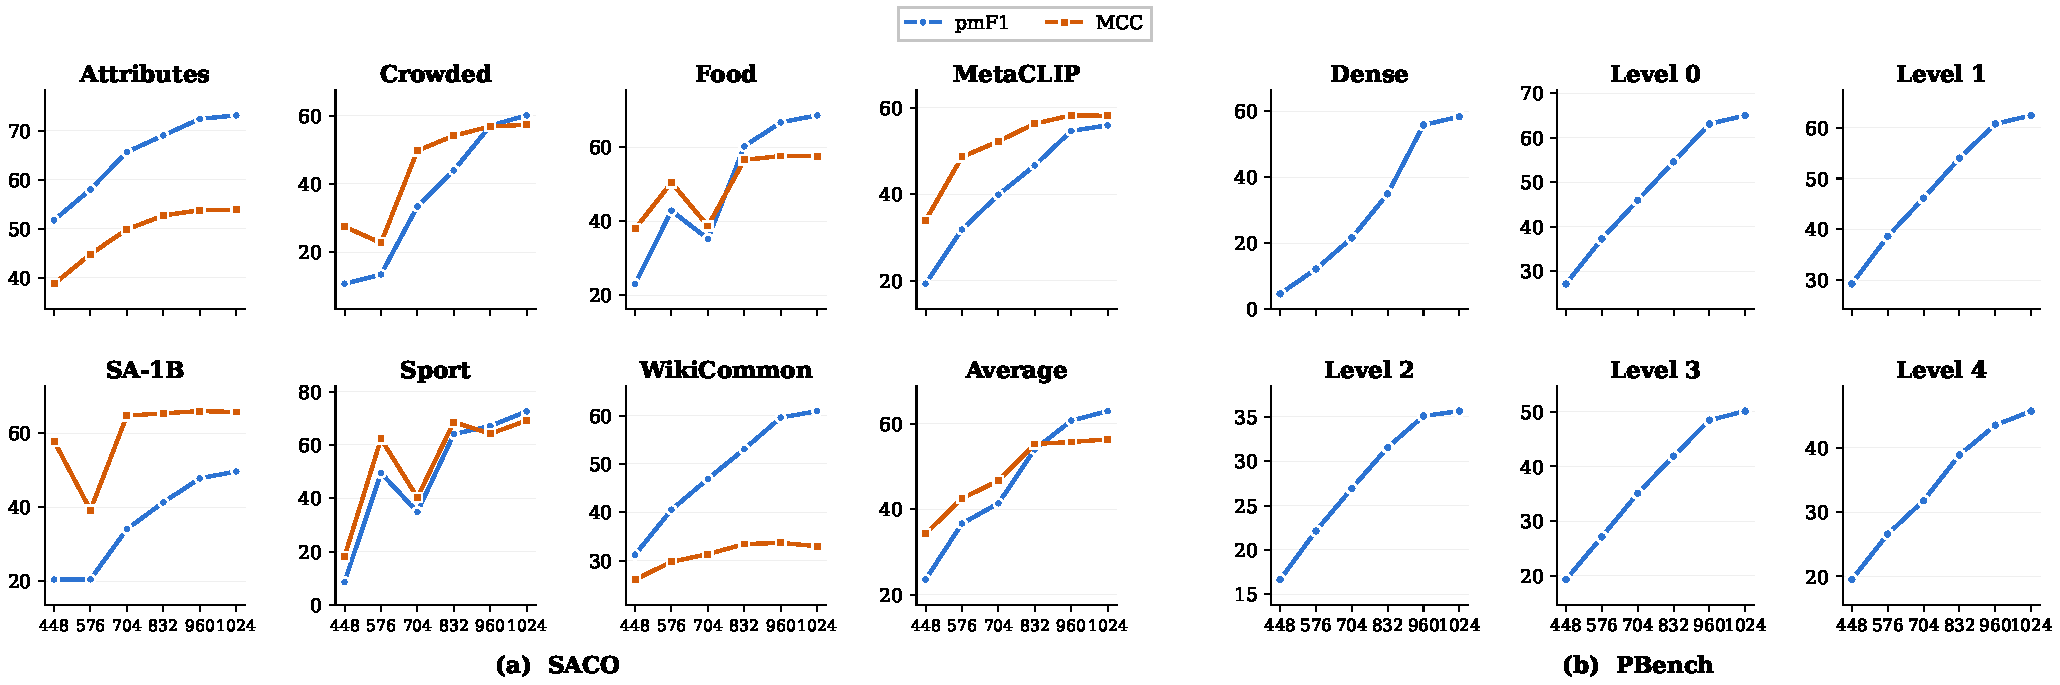
\includegraphics[width=\linewidth]{figures/resolution_all.pdf}
    \caption{\textbf{Resolution Scaling.} Performance as a function of image resolution. While semantic tasks (\eg, Attributes) are relatively robust to lower resolutions, dense and small-object tasks (\eg, Crowded, Sports, Dense) exhibit a phase transition, requiring high resolution to resolve individual instances.}
    \label{fig:resolution}
\end{figure}



\noindent  we observe a  "Dense" phase transition on \textbf{PBench Dense stress test}, where the model is effectively blind at $448^2$ (3.9\% micro-F1) but reaches 61.0\% at $1024^2$. This $\mathbf{15\times}$ improvement confirms that for crowded scenes, while the transformer backbone can understand semantics at low resolution, the "bottleneck" for dense perception is strictly spatial: resolving high details in the input image is a prerequisite for the specialized heads to operate effectively. Furthermore, we notice a decoupling between recognition and grounding. At $448^2$, the model achieves a respectable IL\_MCC of 0.34 (detecting presence) but a poor pmF1 of 23.6 (drawing masks). As resolution increases to $1024^2$, localization quality (pmF1) improves by $\mathbf{2.7\times}$, while classification (MCC) grows more modestly by $\mathbf{1.6\times}$. This suggests that low-resolution features are sufficient for semantic recognition ("is there a cat?"), but high-resolution input is  necessary for precise spatial grounding ("where exactly is the cat?").

\noindent \textbf{Inference Budget (Fixed \vs Adaptive Resizing):} We investigate the trade-off between inference cost and performance by comparing two resizing strategies: (1) \textit{Adaptive ("Smart") Resizing}, where images smaller than $1024^2$ are processed at their native resolution to save compute, and (2) \textit{Fixed Resizing}, where all images are upscaled to $1024^2$.

\begin{figure}[t]
    \centering
    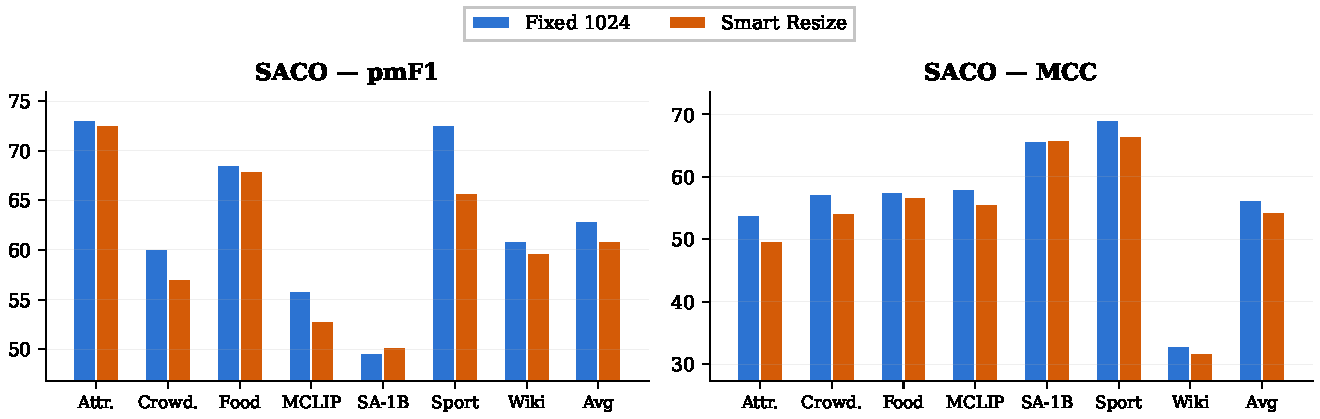
\includegraphics[width=\linewidth]{figures/saco_resize.pdf}
    \caption{\textbf{Resizing Strategy.} Comparison of Adaptive \vs Fixed ($1024^2$) resizing on SA-Co. Upscaling all images to a fixed high resolution consistently improves performance, particularly for crowded scenes.}
    \label{fig:resize_strategy}
\end{figure}

\noindent We find that Fixed Resizing consistently outperforms the adaptive approach, even for images natively smaller than the target resolution. On the SA-Co benchmark, Fixed Resizing yields an average improvement of \textbf{+1.6 pmF1} (63.9 \vs 62.3) and \textbf{+1.6 MCC}. The gain is most pronounced on the \textit{Crowded} split (\textbf{+3.7 pmF1}), suggesting that upscaling small images onto a finer grid is critical for resolving dense clusters and small objects.


\subsection{Effect of Sampling\label{sec:sampling}}

\begin{figure*}[t]
    \centering
    \begin{subfigure}[b]{0.77\textwidth}
        \centering
        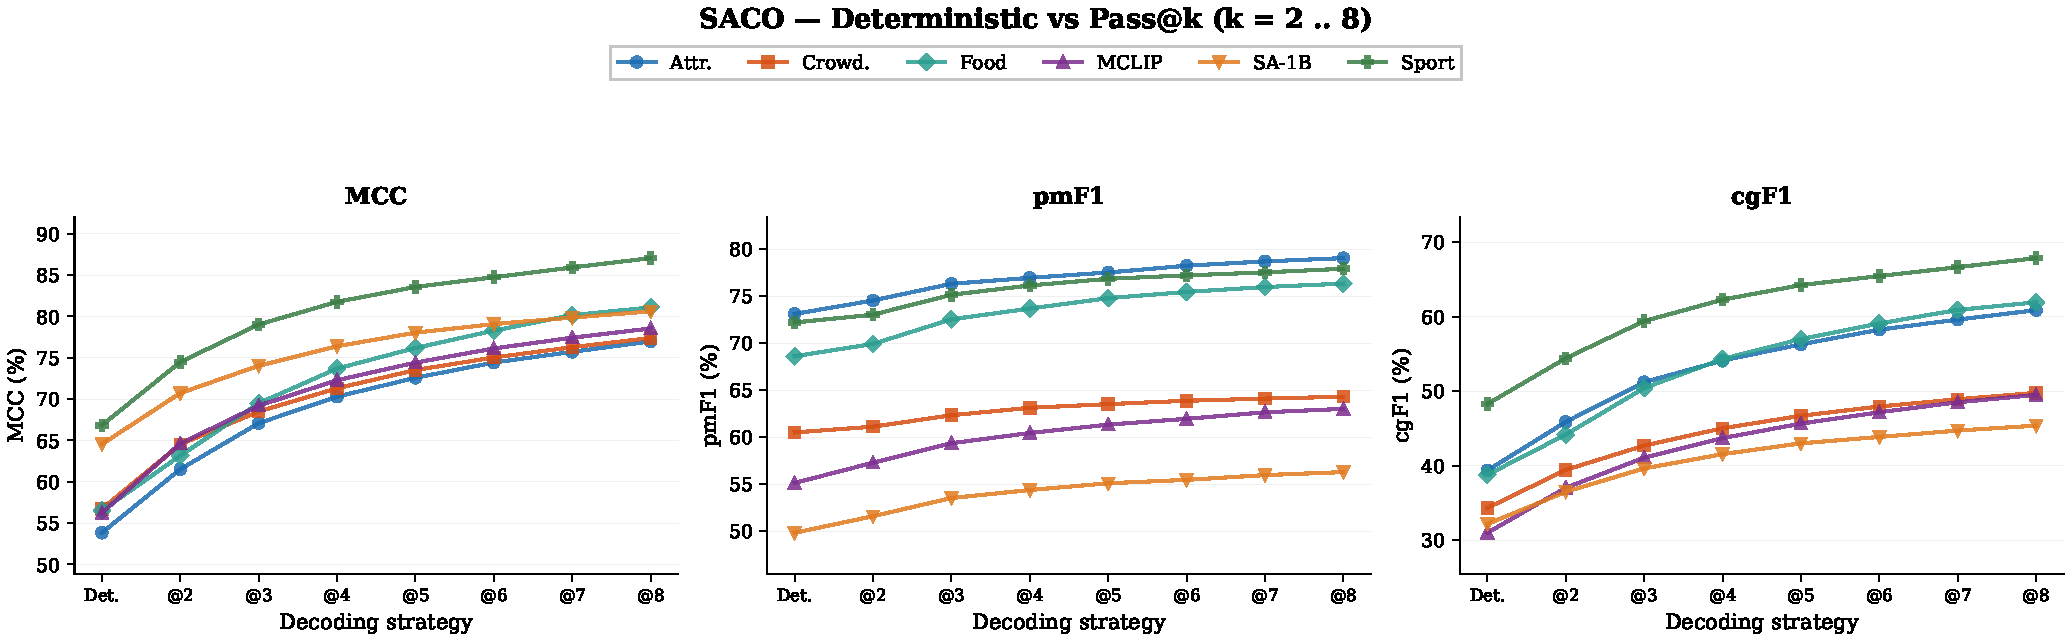
\includegraphics[width=\textwidth, trim=3cm 9cm 3cm 0.1cm, clip]{figures/sampling/sampling_comparison.pdf}\\
        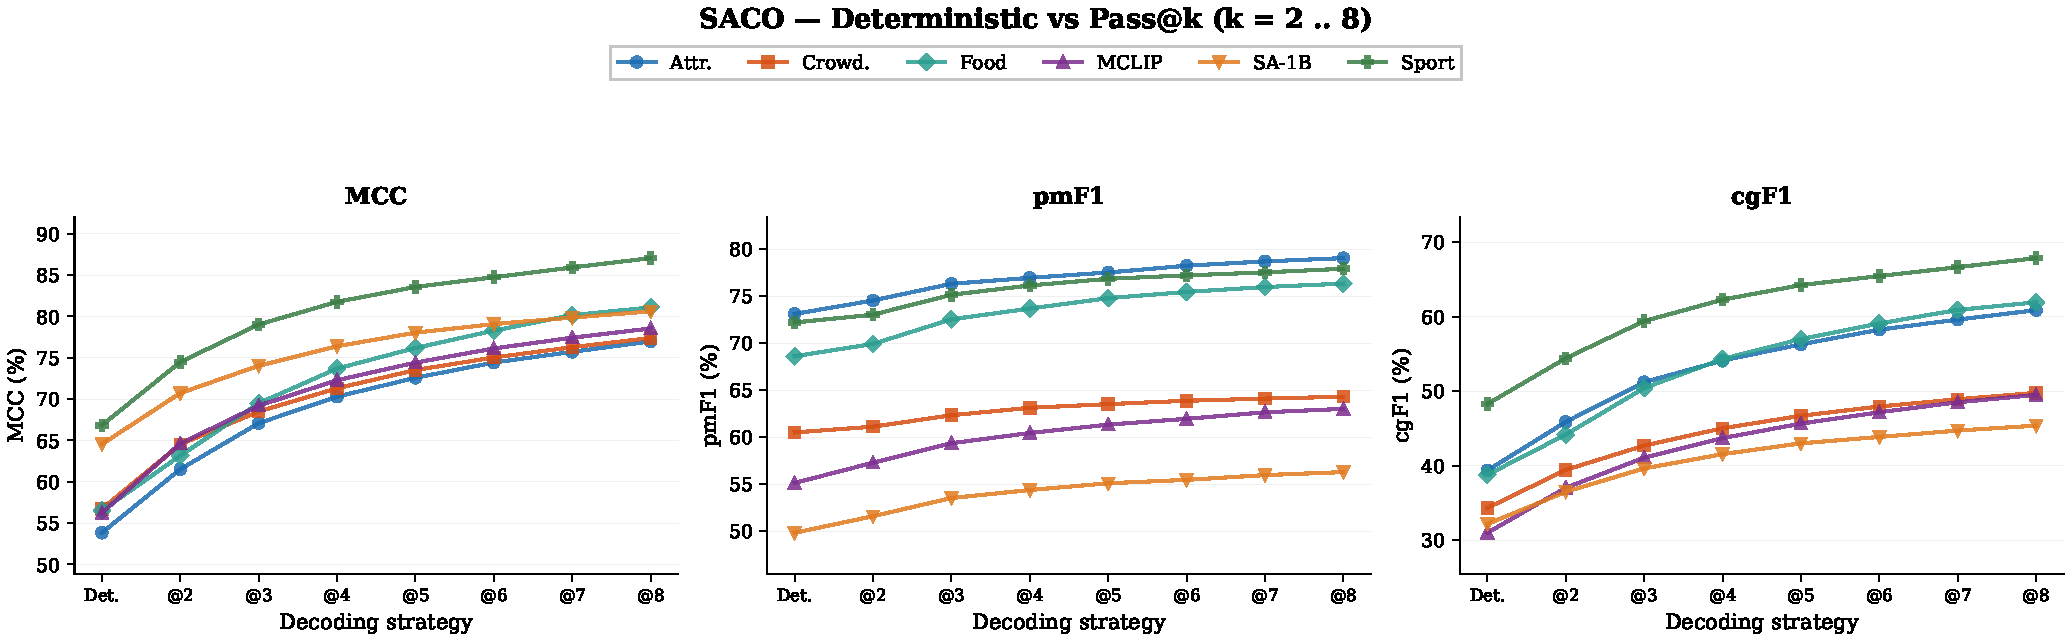
\includegraphics[width=\textwidth, trim=0 0 0 4cm, clip]{figures/sampling/sampling_comparison.pdf}
        \caption{SACO}
        \label{fig:saco_plots}
    \end{subfigure}
    \hfill
    \begin{subfigure}[b]{0.22\textwidth}
        \centering
        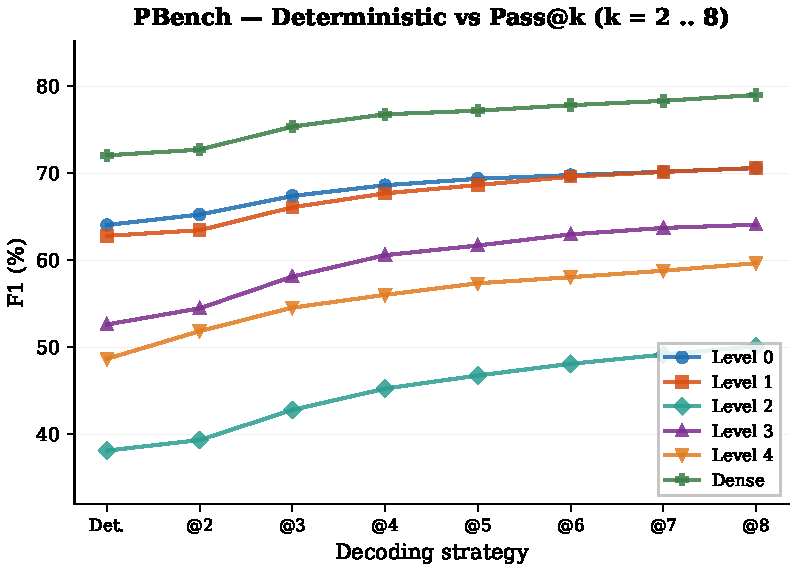
\includegraphics[width=\textwidth]{figures/sampling/pbench_sampling_comparison.pdf}
        \caption{PBench}
        \label{fig:pbench_plots}
    \end{subfigure}
    
    \caption{\textbf{Pass@k Performance scaling.} Evolution of detection metrics across SACO (left) and PBench (right) as the number of samples $k$ increases. Performance consistently scales with $k$, particularly on the most challenging subsets.}
    \label{fig:multipass_plots}
\end{figure*}

To further investigate the latent capabilities of Falcon Perception, we evaluate its performance under a sampling-based inference regime, and report Pass@$k$ (best score out of $k$ predictions). Doing so, we hypothesize that the maximum likelihood objective used during training allows the model to capture a rich distribution of potential outputs, some of which may be more accurate than the most certain prediction in complex scenarios.

\noindent \textbf{Sampling Mechanism:} 
We enable stochastic decoding by sampling from the output heads of the model across three primary dimensions:
\begin{itemize}[nosep]
    \item \textit{Language Head:} We sample from the vocabulary logits, allowing for diversity in the generated tokens. This mainly influences the end of generation, \textit{i.e.}, whether the model decides if there is an object corresponding to the query in the image or not, and how many objects there are to detect and segment.
    \item \textit{Center Head:} We sample from the $x$ and $y$ bin logits, which governs the localization of object centers. Thus, this influences the exact localization of the object and which object to detect at the current timestep. 
    \item \textit{Size Head:} We sample from the $h$ and $w$ bin logits, influencing the predicted dimensions of the bounding boxes.
\end{itemize}

\noindent \textbf{Experimental Protocol:}
We evaluate the model on both the SA-Co and PBench benchmarks. For each test instance, we generate $k$ independent samples and select the "best" prediction (Pass@$k$) based on the task-specific metric. We compare the baseline deterministic (argmax) performance against $k \in \{2, 4, 6, 8\}$.


\begin{wraptable}{r}{0.5\textwidth}
    \centering
    \caption{\textbf{Multi-Pass PBench Benchmark Results.} Comparison of Falcon Perception across different baseline detection passes on PBench levels and dense scenarios against SAM3.}
    \label{tab:pbench_multipass}
    \setlength{\tabcolsep}{6pt}

    \adjustbox{max width=0.5\textwidth}{
    \begin{tabular}{l ccc ccc}
    \toprule
    \textbf{Model} & \textbf{Level 0} & \textbf{Level 1} & \textbf{Level 2} & \textbf{Level 3} & \textbf{Level 4} & \textbf{Dense}\\
    \midrule
    \multicolumn{7}{l}{\cellcolor{gray!10}\textbf{State-of-the-Art}} \\
    SAM 3 & 64.3 & 54.4 & 24.6 & 31.6 & 33.3 & 58.4 \\
    \midrule
    \multicolumn{7}{l}{\cellcolor{gray!10}\textbf{Falcon Perception}} \\
    Det. (baseline) & 64.0 & 62.8 & 38.1 & 52.6 & 48.7 & 72.1\\
    Pass@2        & 65.2 & 63.4 & 39.3 & 54.5 & 51.8 & 72.7 \\
    Pass@4        & 68.6 & 67.7 & 45.2 & 60.6 & 56.0 & 76.8 \\
    Pass@6        & 69.8 & 69.6 & 48.1 & 63.0 & 58.0 & 77.8 \\
    Pass@8        & \textbf{70.6} & \textbf{70.6} & \textbf{50.1} & \textbf{64.1} & \textbf{59.7} & \textbf{79.0} \\
    \bottomrule
    \end{tabular}
    }
\end{wraptable}

\noindent \textbf{Results:} As shown in Table~\ref{tab:saco_multipass} \& ~\ref{tab:pbench_multipass} and Figure~\ref{fig:multipass_plots}, performance across all metrics and subsets consistently improves as $k$ increases. Especially, we note that we outperform the deterministic baseline from pass@$2$.
On the SA-Co benchmark (Table~\ref{tab:saco_multipass}), the average $cgF_1$ score jumps from $34.7$ (Baseline) to $54.3$ (Pass@8), on-par with SAM3, \textit{i.e.}, a \textbf{+19.6} point absolute increase. The most significant delta is observed in the \textit{Wiki-Common} subset, where $cgF_1$ improves from $19.3$ to $45.0$, outperforming SAM3 from pass@$4$. 
On PBench (Table~\ref{tab:pbench_multipass}), we observe a similar trend across all difficulty levels. The "hard" scenarios show the most significant recovery: for \textit{Level 2}, \textit{Level 3}, and \textit{Level 4}, $F_1$ scores increase by \textbf{+12.0}, \textbf{+11.5}, and \textbf{+11.0} points respectively when moving from deterministic to Pass@8.
Furthermore, we find that sampling is particularly effective in "hard" scenes with extreme occlusion, dense object clusters, or expressions requiring complex reasoning. In these instances, the model's first-best prediction might fail, but the underlying probability distribution often contains the correct solution within the top few samples (see Section~\ref{sec:appendix_sampling} for the qualitative analysis).


\begin{table}[t]
    \centering
    \caption{\textbf{Multi-Pass SA-Co Benchmark Results.} Comparison of Falcon Perception across different baseline detection passes against SAM 3.\vspace{-0.2cm}}
    \label{tab:saco_multipass}
    \resizebox{\textwidth}{!}{
    \begin{tabular}{l ccc ccc ccc ccc ccc ccc ccc ccc}
    \toprule
    \multirow{2}{*}{\textbf{Model}} & \multicolumn{3}{c}{\textbf{Average}} & \multicolumn{3}{c}{\textbf{Metaclip}} & \multicolumn{3}{c}{\textbf{SA-1B}} & \multicolumn{3}{c}{\textbf{Crowded}} & \multicolumn{3}{c}{\textbf{Food\&Drink}} & \multicolumn{3}{c}{\textbf{Sports Equip.}} & \multicolumn{3}{c}{\textbf{Attributes}} & \multicolumn{3}{c}{\textbf{Wiki-Common}} \\
    \cmidrule(lr){2-4} \cmidrule(lr){5-7} \cmidrule(lr){8-10} \cmidrule(lr){11-13} \cmidrule(lr){14-16} \cmidrule(lr){17-19} \cmidrule(lr){20-22} \cmidrule(lr){23-25}
    & cgF$_1$ & pmF$_1$ & MCC & cgF$_1$ & pmF$_1$ & MCC & cgF$_1$ & pmF$_1$ & MCC & cgF$_1$ & pmF$_1$ & MCC & cgF$_1$ & pmF$_1$ & MCC & cgF$_1$ & pmF$_1$ & MCC & cgF$_1$ & pmF$_1$ & MCC & cgF$_1$ & pmF$_1$ & MCC \\
    
    \midrule
    \multicolumn{25}{l}{\cellcolor{gray!10}\textbf{State-of-the-Art}} \\
    \quad SAM 3 & 54.2 & 66.1 & \textbf{0.82} & 47.5 & 58.6 & \textbf{0.81} & \textbf{53.8} & \textbf{62.6} & \textbf{0.86} & \textbf{60.9} & \textbf{67.7} & \textbf{0.90} & 53.2 & 67.3 & 0.79 & 65.7 & 73.8 & \textbf{0.89} & 54.7 & 72.0 & 0.76 & 40.2 & 60.9 & \textbf{0.66} \\
    
    \midrule
    \multicolumn{25}{l}{\cellcolor{gray!10}\textbf{Falcon Perception}} \\
    \quad Det. (Baseline) & 34.7 & 62.9 & 0.55 & 31.0 & 55.1 & 0.56 & 32.2 & 49.8 & 0.65 & 34.3 & 60.5 & 0.57 & 38.8 & 68.6 & 0.57 & 48.3 & 72.2 & 0.67 & 39.4 & 73.1 & 0.54 & 19.3 & 60.9 & 0.32 \\
    \quad Pass@2 & 40.5 & 64.6 & 0.63 & 37.0 & 57.3 & 0.65 & 36.5 & 51.6 & 0.71 & 39.4 & 61.1 & 0.65 & 44.2 & 69.9 & 0.63 & 54.4 & 73.0 & 0.74 & 45.9 & 74.5 & 0.62 & 25.8 & 64.9 & 0.40 \\
    \quad Pass@4 & 48.1 & 67.8 & 0.71 & 43.7 & 60.4 & 0.72 & 41.5 & 54.4 & 0.76 & 45.0 & 63.1 & 0.71 & 54.3 & 73.7 & 0.74 & 62.3 & 76.1 & 0.82 & 54.1 & 77.0 & 0.70 & 35.7 & 69.6 & 0.51 \\
    \quad Pass@6 & 51.8 & 68.9 & 0.75 & 47.2 & 62.0 & 0.76 & 43.9 & 55.5 & 0.79 & 47.9 & 63.9 & 0.75 & 59.1 & 75.5 & 0.78 & 65.4 & 77.2 & 0.85 & 58.2 & 78.2 & 0.74 & 41.0 & 70.4 & 0.58 \\
    \quad Pass@8 & \textbf{54.3} & \textbf{69.8} & 0.78 & \textbf{49.5} & \textbf{63.0} & 0.79 & 45.4 & 56.3 & 0.81 & 49.8 & 64.3 & 0.77 & \textbf{61.9} & \textbf{76.3} & \textbf{0.81} & \textbf{67.8} & \textbf{77.9} & 0.87 & \textbf{60.9} & \textbf{79.1} & \textbf{0.77} & \textbf{45.0} & \textbf{71.4} & 0.63 \\
    \bottomrule
    \end{tabular}
    \vspace{-0.2cm}
    }
\end{table}





\subsection{Initialization: Random \texorpdfstring{\vs}{vs} Distillation\label{sec:init_compare}}
Here, we analyze the impact of initializing the Falcon-Perception weights using the multi-teacher distillation, detailed earlier in Sec.~\ref{sec:mtd}. To this end, we pretrain and decay (stages 1 and 2 of our recipe) a smaller 300M-sized model on the detection task (bounding boxes) 
\begin{wrapfigure}{r}{0.5\textwidth}
\centering
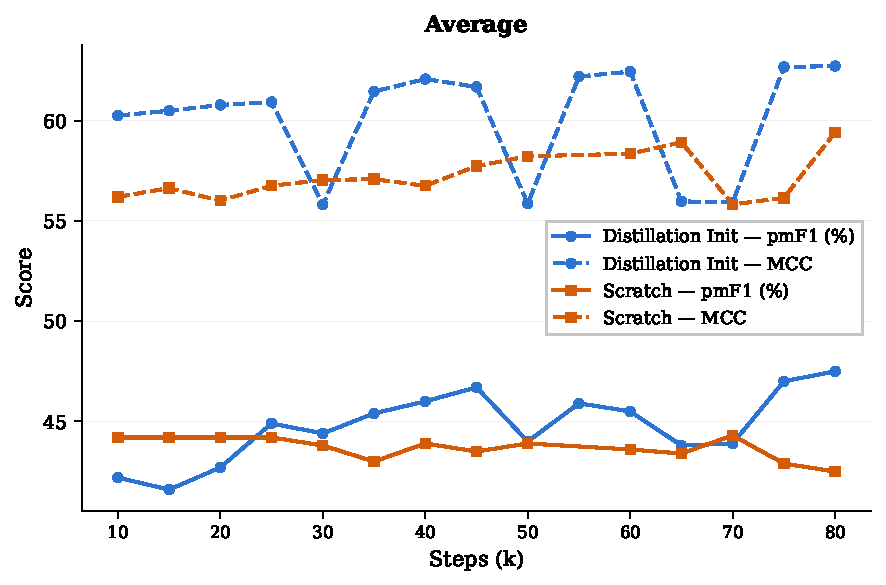
\includegraphics[width=0.8\linewidth]{figures/sweeps/init_compare_avg_combined}
\caption{\textbf{Impact of initialization:} Random weight initialization results in lower performance, compared to distillation initialization, even after being trained long enough for 230K steps over pretraining and decay (stages 1 and 2) combined.\label{fig:distil}}
\end{wrapfigure}
with different weights initialization. From Figure~\ref{fig:distil}, we observe that even after 230K steps of training across both stages, the average performance of randomly initialized model lags the distillation initialized model on the Sa-Co benchmark on both pmF1 and classification (MCC) metrics by a significant margin. Additionally, we note that training with scratch initialization for the segmentation task diverged in the early stages of pretraining itself. This is likely attributed to the fact that accurately predicting the instance masks requires enhanced image features that encode the structure of the scene, which is not possible in early stages of the training with random initialization. Consequently, it results in high gradients for the image tokens leading to divergence of the model weights. Both these ablations clearly indicate the necessity and effectiveness of the multi-teacher distillation stage in our training pipeline. 



